\section{Step-by-step Demonstration}
\label{sec:demo}

\begin{figure}[!t]
\centering
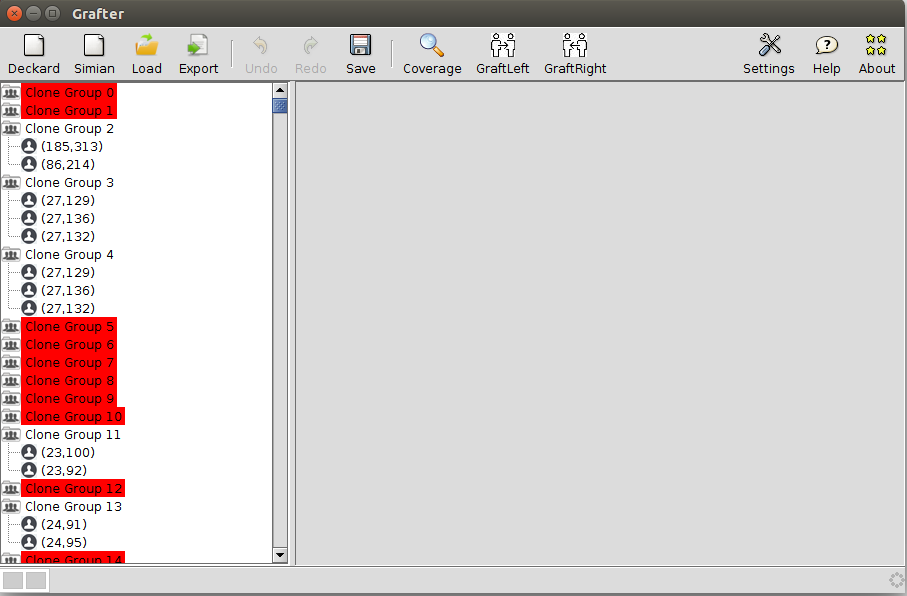
\includegraphics[width=0.5\textwidth]{grafter_new.png}
\caption{Load detected clones and proactively filter out low-quality clones.}
\label{fig:load}
\end{figure}

\subsection{Detect and Load Clones to Grafter}

To ease the effort of detecting clones in a large code base, {\grafter} integrates two clone detection tools, Deckard~\cite{Jiang2007a} and Simian~\cite{simian} (see \ding{172} in Figure~\ref{fig:screenshot}). Deckard parses source code to abstract syntax trees (ASTs) and detects similar code via tree comparison, while Simian is a commercial tool that detects duplicated code via text comparison. Users can also specify the clones of interest in an xml file and load these clones manually by clicking the ``Load'' button.

As noted by previous studies~\cite{bellon2007comparison, roy2009comparison}, clone detection tools may emit a large amount of plausible clones---clones that are syntactically similar but are trivial to analyze. {\grafter} proactively detects such trivial clones using several simple heuristics and marks them in red, as shown in Figure~\ref{fig:load}. {\grafter} considers a group of clones is trivial if (1) clones are in comments or declaration statements, (2) clones are not syntactically complete, or (3) clones are from the same method. {\grafter} also marks clones in test files in red, since {\grafter} aims to contrast the runtime behavior of clones in functional code.

\subsection{Inspect Clones}

Users can inspect the textual differences of loaded clones by right clicking a clone group and select ``Compare'' (see \ding{174} in Figure~\ref{fig:screenshot}). We customized the existing program differencing feature in JMeld to only compute the differences between the cloning regions in two Java files. So users only need to focus on the textual differences between the cloning regions, instead of the entire files. Each clone in the group is named in the format of ``(start line number, end line number)'' by default. Users can update the cloning region or rename it with the method name by double clicking the clone label.

During the manual inspection, if a user considers a clone group to be trivial, she can filter out the clone group by right clicking the group label and select ``Exclude.'' Similary, if a user finds a clone group is mistakenly excluded, she can re-add the group again by right clicking the group label and select ``Include.''

\begin{figure}[!t]
\centering
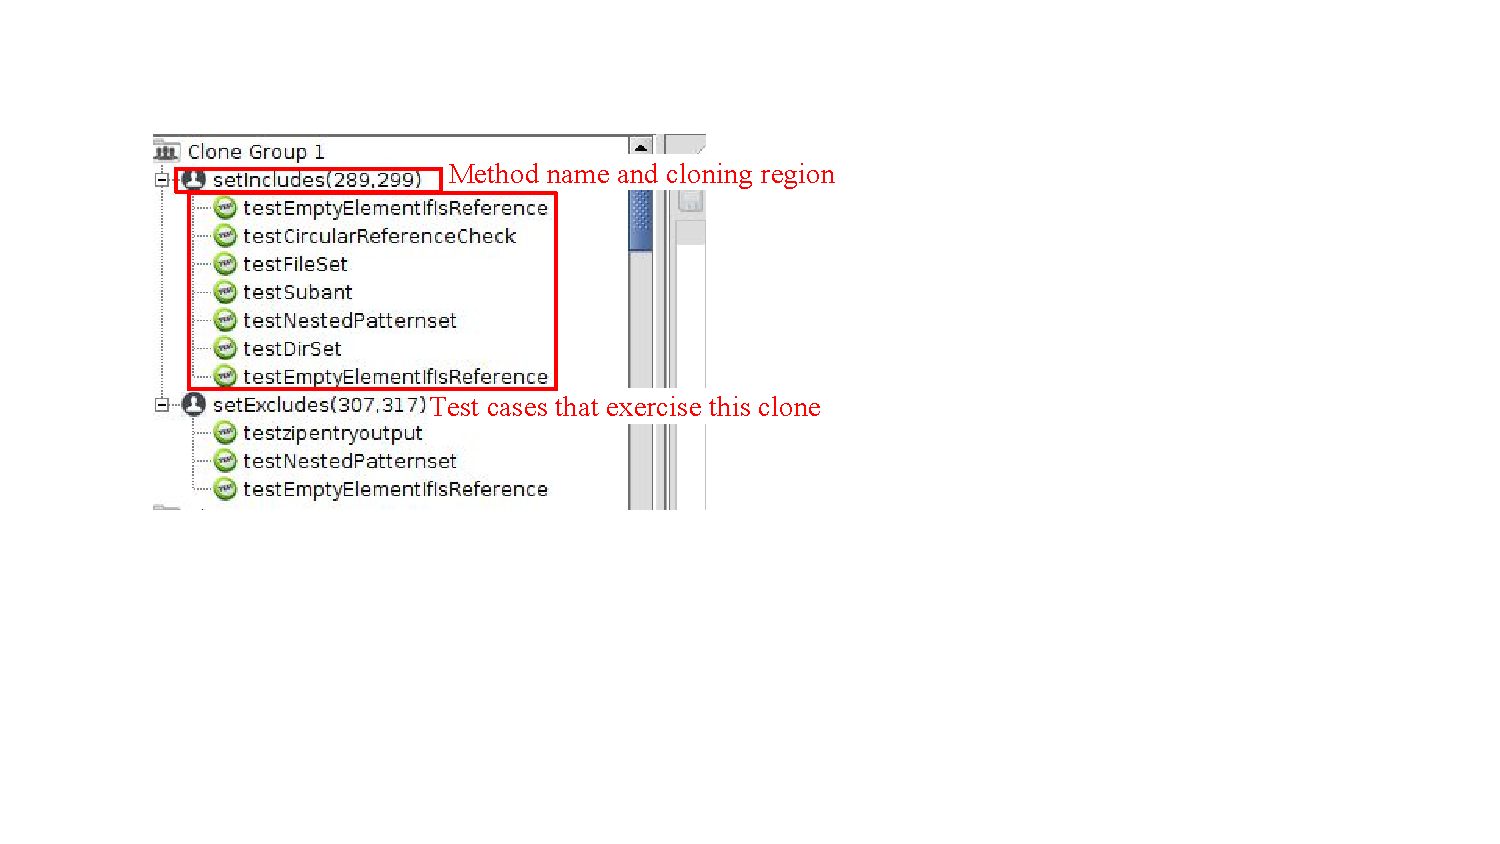
\includegraphics[width=0.45\textwidth]{clone-group-view.pdf}
\caption{The clone group view.}
\label{fig:output}
\end{figure}

\subsection{Find Test Cases of Clones}

When a target project contains a large number of clones and test files, it may not be easy to manually find the test cases for each detected clone. Instead, a user can click the ``Coverage'' button and {\grafter} will automatically locate test cases for each loaded clone (see \ding{173} in Figure~\ref{fig:screenshot}). To analyze the test coverage of code clones, {\grafter} instruments each clone to print out their call stack traces and gathered the test cases appearing in the traces. Note that {\grafter} requires at least one clone in the clone group to be executed by one or more tests in order to reuse tests on its counterpart clones. If none of the clones in a group is covered by a test case, a user should discard the clone group by right clicking and select ``Exclude.''

\subsection{Reuse Tests and Examine Behavioral Differences}

\begin{figure}[!t]
\centering
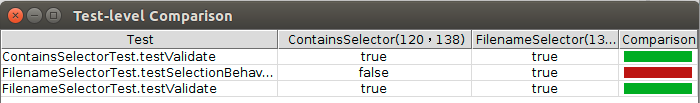
\includegraphics[width=0.5\textwidth]{grafter-test-diff.png}
\caption{The test-level behavior differencing of Grafter}
\label{fig:test}
\end{figure}

\begin{figure}[!t]
\centering
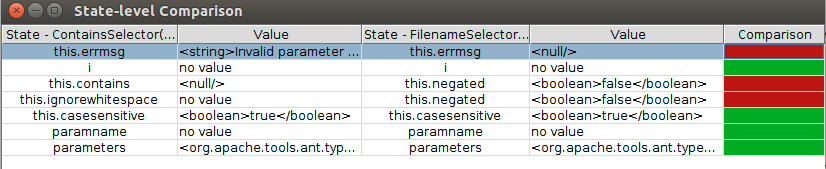
\includegraphics[width=0.5\textwidth]{grafter-state-diff.png}
\caption{The state-level behavior differencing of Grafter}
\label{fig:state}
\end{figure}

\noindent{\bf Test-level Comparison.} Users can compare test outcomes of two clones by right clicking the clone group and selecting ``Compare Test Behavior''. The comparison results are represented in a table and behavioral differences are highlighted in red for ease of investigation, as shown in Figure~\ref{fig:test}. The first column shows names of test cases. The second and third columns show whether each clone passes or fails the corresponding test case. The last column shows the comparison result. Green means both clones are consistent on this test and red means their test outcomes are different.

\noindent{\bf State-level Comparison.} Users can compare intermediate state values of two clones by right clicking the clone group and selecting ``Compare State Behavior''. In the state-level comparison table in Figure~\ref{fig:state}, the first and third columns show the name of corresponding variables referenced by code clones, and the second and fourth columns show the values of variables in the format of XML. {\grafter} prints the value of an object in XML using XStream. Users can view the complete xml representation of an object by hovering the mouse over the corresponding cell, as shown in Figure~\ref{fig:hover}.

\begin{figure}[!t]
\centering
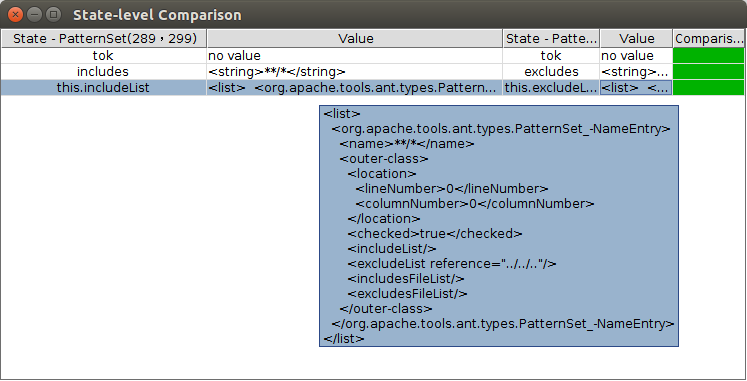
\includegraphics[width=0.45\textwidth]{hover.png}
\caption{Inspect the intermediate state value.}
\label{fig:hover}
\end{figure}

\subsection{Inspecting Grafted Clone} 

Note that the inserted stub code doesn't persist during test transplantation and therefore doesn't need to be comprehended by the developers. Yet {\grafter}'s GUI still allows users to experiment with clone grafting and inspect the intermediate grafted code. Users can graft the left clone to replace the right one and view the grafted code in the diff view by clicking ``Graft Left'' in the top menu bar (vice versa). Users can further test the grafted code by right clicking the clone group and select ``Test''. Users can undo and redo the previous graft by clicking the "Undo" and "Redo" buttons on the top menu bar respectively.

\begin{figure}[!t]
\centering
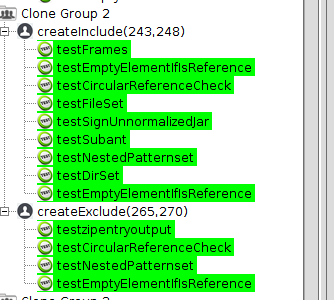
\includegraphics[width=0.4\textwidth]{test-grafted-clone.png}
\caption{Test the grafted clone.}
\label{fig:hover}
\end{figure}